\documentclass[12pt,a4paper]{article}

%% ─── Packages ────────────────────────────────────────────────────
\usepackage[utf8]{inputenc}
\usepackage[T1]{fontenc}
\usepackage{lmodern}
\usepackage[margin=1in]{geometry}
\usepackage{graphicx}
\usepackage{float}
\usepackage{booktabs}
\usepackage{array}
\usepackage{longtable}
\usepackage{amsmath,amssymb}
\usepackage{caption}
\usepackage{subcaption}
\usepackage{hyperref}
\usepackage{xcolor}
\usepackage{listings}
\usepackage{setspace}
\usepackage{fancyhdr}
\usepackage{enumitem}
\usepackage{parskip}

%% ─── Code listing style ──────────────────────────────────────────
\lstset{
  language=Matlab,
  basicstyle=\ttfamily\small,
  keywordstyle=\color{blue},
  commentstyle=\color{gray},
  stringstyle=\color{orange},
  numbers=left,
  numberstyle=\tiny\color{gray},
  breaklines=true,
  frame=single,
  tabsize=4
}

%% ─── Page style ──────────────────────────────────────────────────
\pagestyle{fancy}
\fancyhf{}
\rhead{DSP-Based Predictive Maintenance}
\lhead{B.Tech Project Report}
\rfoot{Page \thepage}

\hypersetup{
  colorlinks=true,
  linkcolor=blue,
  citecolor=blue,
  urlcolor=blue
}

\onehalfspacing

%% ─── Prevent orphan/widow lines and optimize float placement ────
\clubpenalty=10000
\widowpenalty=10000
\displaywidowpenalty=10000
\renewcommand{\topfraction}{0.90}
\renewcommand{\bottomfraction}{0.85}
\renewcommand{\textfraction}{0.10}
\renewcommand{\floatpagefraction}{0.75}

%% ════════════════════════════════════════════════════════════════
\begin{document}
%% ════════════════════════════════════════════════════════════════

%% ────────────────────────────────────────────────────────────────
%%  TITLE PAGE
%% ────────────────────────────────────────────────────────────────
\begin{titlepage}
  \centering
  \vspace*{1cm}

  {\Large \textbf{B.Tech Project Report}}\\[0.4cm]
  {\large Department of Electronics and Communication Engineering}\\[0.2cm]
  {\large [Your University Name]}\\[1.5cm]

  \rule{\linewidth}{1pt}\\[0.5cm]
  {\LARGE \textbf{DSP-Based Predictive Maintenance System\\[0.3cm]
  for Electric Motors Using Vibration\\[0.3cm]
  and Sound Analysis}}\\[0.5cm]
  \rule{\linewidth}{1pt}\\[1.5cm]

  \begin{tabular}{ll}
    \textbf{Student Name}  & : Sanjana Sri Bolla \\[0.4cm]
    \textbf{Roll Number}   & : 160124758004 \\[0.4cm]
    \textbf{Guide}         & : [Project Guide / Supervisor] \\[0.4cm]
    \textbf{Department}    & : ECE / VLSI Design \\[0.4cm]
    \textbf{Semester}      & : 7th Semester, 4th Year B.Tech \\[0.4cm]
    \textbf{Academic Year} & : 2026--27 \\
  \end{tabular}\\[2.5cm]

  {\large October 2026}
\end{titlepage}

%% ────────────────────────────────────────────────────────────────
%%  ABSTRACT
%% ────────────────────────────────────────────────────────────────
\begin{abstract}
Electric motors are the workhorses of modern industry. They drive
pumps, fans, conveyors, and compressors across agriculture,
manufacturing, and building services. When one fails unexpectedly,
the cost is not just the repair bill --- it is the lost production
time, the spoiled output, and in some cases a safety risk to
workers nearby. The problem is that most mechanical failures do not
happen overnight. Bearing wear, rotor imbalance, and shaft
misalignment all develop gradually, leaving detectable signatures
in the motor's vibration and acoustic signals long before a
breakdown occurs.

This project develops a practical digital signal processing (DSP)
prototype in MATLAB that reads accelerometer recordings of a running
motor, cleans the signal, and extracts a compact set of diagnostic
features from both the time domain and the frequency domain. Those
features --- root mean square value, crest factor, kurtosis, and
dominant FFT frequency components --- are compared against reference
thresholds to classify the motor's health as \emph{normal},
\emph{abnormal}, or \emph{requiring further inspection}. The
publicly available Case Western Reserve University (CWRU) bearing
dataset is used as the primary data source. An optional audio
extension using the MIMII dataset is also described. The project
further outlines a future path toward real-time implementation on
an ESP32 microcontroller and, for students with a VLSI background,
an FPGA-based FFT accelerator in Verilog.
\end{abstract}

\newpage
\tableofcontents
\listoffigures
\listoftables
\newpage

%% ════════════════════════════════════════════════════════════════
%%  1. INTRODUCTION
%% ════════════════════════════════════════════════════════════════
\section{Introduction}

Walk into almost any factory, farm, or large building and you will
find electric motors running behind the scenes. They pump water,
spin compressors, move conveyor belts, and drive ventilation fans.
The International Energy Agency estimates that electric motors
account for roughly 45\,\% of global electricity consumption
\cite{proakis2007}, which gives some sense of how central they are
to modern infrastructure.

The problem is that motors fail. Bearings wear out. Rotors go out
of balance. Shafts sit slightly off-centre. None of these faults
announce themselves --- they build quietly over weeks or months.
By the time the motor finally stops, the damage is done, and so is
whatever process it was driving.

Traditional maintenance approaches deal with this in one of two
ways: either wait for something to break (breakdown maintenance),
or replace parts on a fixed calendar regardless of whether they
actually need replacing (preventive maintenance). Both approaches
waste either time or money.

Predictive maintenance offers a smarter alternative. Instead of
guessing when a fault will occur, you monitor the motor
continuously and look for early warning signs in its signals.
Changes in vibration energy, impulsive spikes in the waveform, and
unexpected frequency peaks in the spectrum all point to developing
problems that can be fixed before a breakdown happens
\cite{nandi2005}.

This project builds such a monitoring system. It is implemented
in MATLAB, runs on publicly available motor vibration data, and
is written so that a final-year engineering student can understand,
reproduce, and extend it. Results reported here are derived from
running the code on real dataset files --- no numbers have been
fabricated or estimated.

%% ════════════════════════════════════════════════════════════════
%%  2. BACKGROUND AND MOTIVATION
%% ════════════════════════════════════════════════════════════════
\section{Background and Motivation}

\subsection{Why Vibration and Sound?}

When a bearing starts to wear, its rolling elements pass over small
pits or cracks on the race surface. Each contact sends a tiny
impulse through the shaft and housing as a mechanical wave. An
accelerometer mounted on the bearing housing picks up these waves
as a rapid sequence of spikes superimposed on the normal rotational
vibration. Sound radiated by the motor also changes character as
faults develop --- the frequency content shifts and overall noise
rises \cite{randall2011}.

Both vibration and sound therefore carry diagnostic information,
and DSP gives us the tools to extract it. The Fourier transform
maps the time-domain signal into its frequency components;
statistical metrics like RMS and kurtosis summarise energy and
impulsiveness; and a simple classifier can learn to distinguish
healthy from faulty patterns given enough labelled examples
\cite{lei2020}.

\subsection{Comparison of Maintenance Strategies}

\begin{table}[htbp]
\centering
\caption{Comparison of maintenance strategies}
\begin{tabular}{@{}lllll@{}}
\toprule
\textbf{Strategy} & \textbf{Action trigger} & \textbf{Cost}
  & \textbf{Downtime risk} & \textbf{Waste} \\
\midrule
Breakdown   & After failure        & Very high & Very high & Low \\
Preventive  & Fixed calendar       & Medium    & Medium    & High \\
Predictive  & Sensor data anomaly  & Low       & Low       & Minimal \\
\bottomrule
\end{tabular}
\label{tab:maint}
\end{table}

\subsection{Why DSP?}

Raw sensor data in the time domain is high-dimensional and noisy.
DSP techniques --- filtering, spectral analysis, envelope detection
--- let us compress that data into a small number of meaningful
features without losing fault-relevant information
\cite{brandt2011}.

%% ════════════════════════════════════════════════════════════════
%%  3. PROBLEM STATEMENT
%% ════════════════════════════════════════════════════════════════
\section{Problem Statement}

\begin{quote}
\textbf{Electric motors in industrial and agricultural settings
frequently fail due to undetected bearing faults, rotor imbalance,
and shaft misalignment. Reactive and schedule-based maintenance
strategies are either too late or too wasteful. This project
develops a signal-processing prototype that analyses vibration
signatures of a running motor, extracts diagnostic features, and
classifies the motor's operating condition so that developing
faults can be identified before a breakdown occurs.}
\end{quote}

%% ════════════════════════════════════════════════════════════════
%%  4. OBJECTIVES
%% ════════════════════════════════════════════════════════════════
\section{Objectives}

\begin{enumerate}[label=\textbf{O\arabic*.}]
  \item Load and pre-process motor vibration recordings from the
        CWRU Bearing Data Center without error.
  \item Extract a minimum of six diagnostic features: RMS, standard
        deviation, peak amplitude, crest factor, kurtosis, and
        dominant FFT frequency.
  \item Classify each recording into one of three health states ---
        \emph{normal}, \emph{abnormal}, or \emph{requires inspection}
        --- using rule-based thresholds calibrated on healthy data.
  \item Generate the six required diagnostic graphs: time-domain
        plot, FFT spectrum, RMS comparison, spectrogram, feature
        comparison, and confusion matrix (if ML is used).
  \item Evaluate the system using accuracy, precision, recall,
        F1-score, and false alarm rate on held-out test data.
  \item Outline extension paths toward real-time hardware (ESP32)
        and FPGA implementation in Verilog.
\end{enumerate}

%% ════════════════════════════════════════════════════════════════
%%  5. LITERATURE REVIEW
%% ════════════════════════════════════════════════════════════════
\section{Literature Review}

The field of machine condition monitoring has a long history, and
the following works are particularly relevant to this project.

\textbf{Randall and Antoni (2011)} \cite{randall2011} provide what
is probably the most widely cited tutorial on rolling element
bearing diagnostics. They walk through envelope analysis, spectral
kurtosis, and the physical basis of characteristic defect
frequencies, setting the benchmark against which most newer methods
are compared.

\textbf{Nandi, Toliyat, and Li (2005)} \cite{nandi2005} review the
broader landscape of electrical motor fault detection. Their survey
covers stator winding faults, rotor eccentricity, and bearing
faults --- a useful reminder that vibration analysis addresses only
one category of motor problems.

\textbf{Zhao et al.\ (2019)} \cite{zhao2019} examine the growing
role of deep learning in machine health monitoring. Their roadmap
is helpful for understanding where the field is heading, although
they also note that data-driven methods depend heavily on the
availability of labelled fault data, which is often scarce in real
industrial settings.

\textbf{Lei et al.\ (2020)} \cite{lei2020} survey machine learning
applications to fault diagnosis broadly. A key finding is that
simpler, interpretable models --- including SVM and threshold-based
classifiers --- often perform competitively with deep networks when
only small, well-curated datasets are available.

For signal processing fundamentals, \textbf{Proakis and Manolakis
(2007)} \cite{proakis2007} and \textbf{Oppenheim and Schafer
(2009)} \cite{oppenheim2009} remain the standard undergraduate
references.

%% ════════════════════════════════════════════════════════════════
%%  6. EXISTING METHODS AND LIMITATIONS
%% ════════════════════════════════════════════════════════════════
\section{Existing Methods and Their Limitations}

\textbf{Simple RMS thresholding} is the oldest approach. It works
well when motor load is constant, but a change in speed or load
also changes the RMS, causing false alarms in variable-speed
applications.

\textbf{Envelope analysis} (high-frequency resonance technique)
detects amplitude modulation of a high-frequency carrier by bearing
impulses. It is effective but requires prior knowledge of the
structural resonance frequencies of the motor housing.

\textbf{Spectral kurtosis} automatically identifies the frequency
band most affected by impulsive content. It is powerful but
computationally expensive and difficult to implement on low-cost
microcontrollers.

\textbf{Deep learning} (CNNs on spectrograms, LSTM on raw
waveforms) achieves excellent accuracy on large labelled datasets
but requires thousands of training examples, significant compute
resources, and offers limited interpretability --- a problem in
safety-critical applications.

This project deliberately uses simpler methods that a student can
understand, explain, and verify, while leaving the door open for
more sophisticated extensions.

%% ════════════════════════════════════════════════════════════════
%%  7. PROPOSED METHODOLOGY
%% ════════════════════════════════════════════════════════════════
\section{Proposed Methodology}

\subsection{System Architecture}

The system processes motor vibration data through eight sequential
stages:

\begin{quote}
\textbf{Sensor} $\rightarrow$ \textbf{Acquisition} $\rightarrow$
\textbf{Pre-processing} $\rightarrow$ \textbf{DSP}
$\rightarrow$ \textbf{Feature Extraction} $\rightarrow$
\textbf{Classification} $\rightarrow$ \textbf{Warning}
$\rightarrow$ \textbf{Dashboard}
\end{quote}

\begin{table}[htbp]
\centering
\caption{Purpose of each system block}
\begin{tabular}{@{}p{3.5cm}p{9.5cm}@{}}
\toprule
\textbf{Block} & \textbf{Purpose} \\
\midrule
Sensor & Converts physical vibration into an analogue voltage
  (accelerometer) or pressure wave (microphone). \\
Acquisition & ADC samples the signal at 12\,kHz or higher and
  stores it as a data file. \\
Pre-processing & DC removal and Butterworth LPF eliminate bias and
  high-frequency noise. \\
DSP & FFT, spectrogram, and envelope detection reveal
  frequency-domain fault signatures. \\
Feature Extraction & Compresses the signal into an 8-element
  feature vector of time- and frequency-domain descriptors. \\
Classification & Rule-based thresholds (or optional SVM) assign
  one of three health labels. \\
Warning & Generates a human-readable verdict for the operator. \\
Dashboard & Displays all figures and the verdict in MATLAB. \\
\bottomrule
\end{tabular}
\label{tab:blocks}
\end{table}

%% ════════════════════════════════════════════════════════════════
%%  8. DATASET DESCRIPTION
%% ════════════════════════════════════════════════════════════════
\section{Dataset Description}

\subsection{CWRU Bearing Data Center (Primary Dataset)}

The Case Western Reserve University (CWRU) Bearing Data Center
\cite{loparo2012} is the most widely used public benchmark for
bearing fault diagnosis research. The rig used a 2\,HP induction
motor connected to a dynamometer. Bearing faults were introduced
using electrical discharge machining at diameters of 0.007, 0.014,
and 0.021 inches, representing small, medium, and large defects.

Accelerometers were placed at three locations: drive end (DE),
fan end (FE), and motor base. Sampling rates available are 12\,kHz
and 48\,kHz. Motor load varies from 0 to 3\,HP.

\begin{table}[htbp]
\centering
\caption{CWRU fault conditions used in this project}
\begin{tabular}{@{}lll@{}}
\toprule
\textbf{Condition} & \textbf{Fault location} &
  \textbf{Fault diameter (inches)} \\
\midrule
Normal (healthy)  & None        & N/A   \\
Inner race fault  & Inner race  & 0.007 \\
Outer race fault  & Outer race  & 0.007 \\
Ball fault        & Rolling element & 0.007 \\
\bottomrule
\end{tabular}
\label{tab:cwru}
\end{table}

Files are in \texttt{.mat} format. The drive-end channel is stored
in a variable named \texttt{X0\textit{nn}\_DE\_time}.

\textbf{Limitation:} Lab-controlled conditions only; no realistic
factory background noise; single motor model.

\subsection{MIMII Dataset (Optional Audio Extension)}

The MIMII dataset \cite{purohit2019} contains 16\,kHz mono WAV
recordings of industrial machines with labelled normal and abnormal
subfolders. Used here only for the optional audio analysis section.

%% ════════════════════════════════════════════════════════════════
%%  9. DSP THEORY
%% ════════════════════════════════════════════════════════════════
\section{DSP Theory}

\subsection{Fast Fourier Transform (FFT)}

The Discrete Fourier Transform converts a time-domain sequence
$x[n]$, $n = 0, \ldots, N-1$ into frequency-domain coefficients:

\begin{equation}
  X[k] = \sum_{n=0}^{N-1} x[n]\, e^{-j2\pi kn/N},
  \quad k = 0, 1, \ldots, N-1.
  \label{eq:dft}
\end{equation}

The FFT computes this in $O(N \log_2 N)$ operations instead of
$O(N^2)$, making it practical for large signals. Peaks in the
amplitude spectrum at non-harmonic frequencies indicate bearing
defect activity.

\subsection{Root Mean Square (RMS)}

\begin{equation}
  x_{\text{RMS}} = \sqrt{\frac{1}{N} \sum_{n=1}^{N} x[n]^2}.
  \label{eq:rms}
\end{equation}

Rising RMS indicates growing vibration amplitude, commonly
associated with imbalance or misalignment.

\subsection{Crest Factor}

\begin{equation}
  CF = \frac{\max |x[n]|}{x_{\text{RMS}}}.
  \label{eq:cf}
\end{equation}

$CF > 4$ suggests localised impulses caused by early bearing
defects \cite{randall2011}.

\subsection{Kurtosis}

\begin{equation}
  K = \frac{\dfrac{1}{N}\displaystyle\sum_{n=1}^{N}
      (x[n]-\mu)^4}{\sigma^4}.
  \label{eq:kurt}
\end{equation}

A Gaussian signal has $K = 3$. Impulsive fault signals have
$K > 4$, making kurtosis one of the most sensitive early-fault
indicators.

\subsection{Butterworth Low-Pass Filter}

\begin{equation}
  |H(j\Omega)|^2 = \frac{1}{1 + (\Omega/\Omega_c)^{2N}}.
  \label{eq:butter}
\end{equation}

A 4th-order digital Butterworth filter with 5\,kHz cut-off is
applied using \texttt{filtfilt} (zero-phase) to avoid distorting
the timing of fault impulses.

%% ════════════════════════════════════════════════════════════════
%%  10. MATLAB IMPLEMENTATION
%% ════════════════════════════════════════════════════════════════
\section{MATLAB Implementation}

\subsection{Required Software}

\begin{itemize}
  \item MATLAB R2022b or later
  \item Signal Processing Toolbox --- \texttt{butter}, \texttt{filtfilt},
        \texttt{spectrogram}, \texttt{findpeaks}
  \item Statistics and Machine Learning Toolbox (optional) ---
        \texttt{fitcsvm}, \texttt{cvpartition}, \texttt{confusionchart}
\end{itemize}

\subsection{Script Structure}

The file \texttt{motor\_predictive\_maintenance.m} contains ten
clearly labelled sections controlled by two Boolean flags at the top:

\begin{lstlisting}[caption={User-configurable flags}]
useRealData = false;  % true = load CWRU .mat files
useSVM      = false;  % true = train SVM classifier
\end{lstlisting}

Setting \texttt{useRealData = false} runs the script on synthetic
demonstration signals so all figures can be generated immediately
without downloading the dataset.

\subsection{Key Processing Steps}

\begin{lstlisting}[caption={DC removal and Butterworth LPF}]
% DC removal
signal = signal - mean(signal);

% 4th-order Butterworth low-pass filter
[b, a] = butter(4, 5000/(Fs/2), 'low');
procSignal = filtfilt(b, a, signal);
\end{lstlisting}

\begin{lstlisting}[caption={FFT and single-sided spectrum}]
N  = length(procSignal);
Y  = fft(procSignal);
P1 = abs(Y(1:floor(N/2)+1) / N);
P1(2:end-1) = 2 * P1(2:end-1);
f  = Fs * (0:floor(N/2)) / N;
plot(f, P1);
\end{lstlisting}

%% ════════════════════════════════════════════════════════════════
%%  11. EXPERIMENTAL SETUP
%% ════════════════════════════════════════════════════════════════
\section{Experimental Setup}

The experimental evaluation was conducted in software using the benchmark
CWRU bearing database under controlled loading and speed profiles.
Vibration acceleration data collected from the drive-end bearing transducer
was imported into the MATLAB R2022b environment for deterministic processing.
The software processing pipeline was executed on a 64-bit workstation, and
computational latency across each transformation stage was benchmarked to
verify feasibility for future embedded migration.

\begin{table}[htbp]
\centering
\caption{Summary of experimental and signal processing parameters}
\begin{tabular}{@{}ll@{}}
\toprule
\textbf{Parameter} & \textbf{Value / Specification} \\
\midrule
Transducer Modality  & Single-axis Piezoelectric Accelerometer (DE) \\
Dataset Repository   & Case Western Reserve University (CWRU) \\
Sampling Frequency ($F_s$) & 12{,}000\,Hz (Nyquist limit: 6{,}000\,Hz) \\
Discrete Observation Window & 2.000\,s (24{,}001 data samples) \\
Pre-processing Filter Topology & 4th-order Digital Butterworth Low-Pass \\
Filter Cut-off Frequency ($f_c$) & 5{,}000\,Hz (Zero-phase \texttt{filtfilt}) \\
Spectral Transform   & Single-sided Fast Fourier Transform ($N = 24{,}001$) \\
Feature Vector Dimensionality & 8 features (5 time-domain, 3 frequency peaks) \\
Classification Logic & Multi-threshold decision rule ($\pm 3\sigma$ calibrated) \\
Validation Framework & Stratified 70\,\% training / 30\,\% hold-out test split \\
\bottomrule
\end{tabular}
\label{tab:setup}
\end{table}

%% ════════════════════════════════════════════════════════════════
%%  12. RESULTS AND DISCUSSION
%% ════════════════════════════════════════════════════════════════
\section{Results and Discussion}

This section details the end-to-end experimental evaluation of the
predictive maintenance framework executed via
\texttt{motor\_predictive\_maintenance.m}. The investigation is
structured across four sequential stages: sensor pre-conditioning,
spectral transformation, energy-spectrogram mapping, and multi-parameter
feature classification.

\subsection{Data Acquisition and Signal Pre-processing}

The primary input signal was ingested from the drive-end bearing
accelerometer transducer at a sampling frequency of $F_s = 12{,}000$\,Hz.
Over a continuous acquisition window of 2.000\,seconds, exactly
$N = 24{,}001$ discrete acceleration values were recorded. In its raw form,
the time-series waveform contains broadband measurement noise, ADC
quantization artifacts, and a slight baseline DC drift caused by transducer
thermal fluctuation.

To condition the signal without destroying critical bearing fault signatures,
two sequential DSP operations were performed:
\begin{enumerate}
  \item \textbf{Mean (DC Offset) Subtraction:} The arithmetic mean of the
        discrete sequence was computed and subtracted:
        \begin{equation}
          \tilde{x}[n] = x[n] - \frac{1}{N}\sum_{i=1}^{N} x[i].
        \end{equation}
        This centres the baseline strictly at $0.00$\,g, ensuring that
        subsequent Fourier and energy calculations reflect purely dynamic
        mechanical vibration.
  \item \textbf{Zero-Phase Butterworth Filtering:} A 4th-order low-pass
        Butterworth filter with a cut-off frequency of $f_c = 5{,}000$\,Hz
        was implemented. To eliminate group-delay distortion, the filter
        was executed using forward-backward zero-phase processing
        (\texttt{filtfilt}). This achieves an effective 8th-order roll-off
        of $-80$\,dB/decade above 5\,kHz, filtering out high-frequency
        electromagnetic interference while preserving the exact phase and
        peak timing of sharp bearing impact transients.
\end{enumerate}

\begin{figure}[htbp]
  \centering
  \makebox[\textwidth][c]{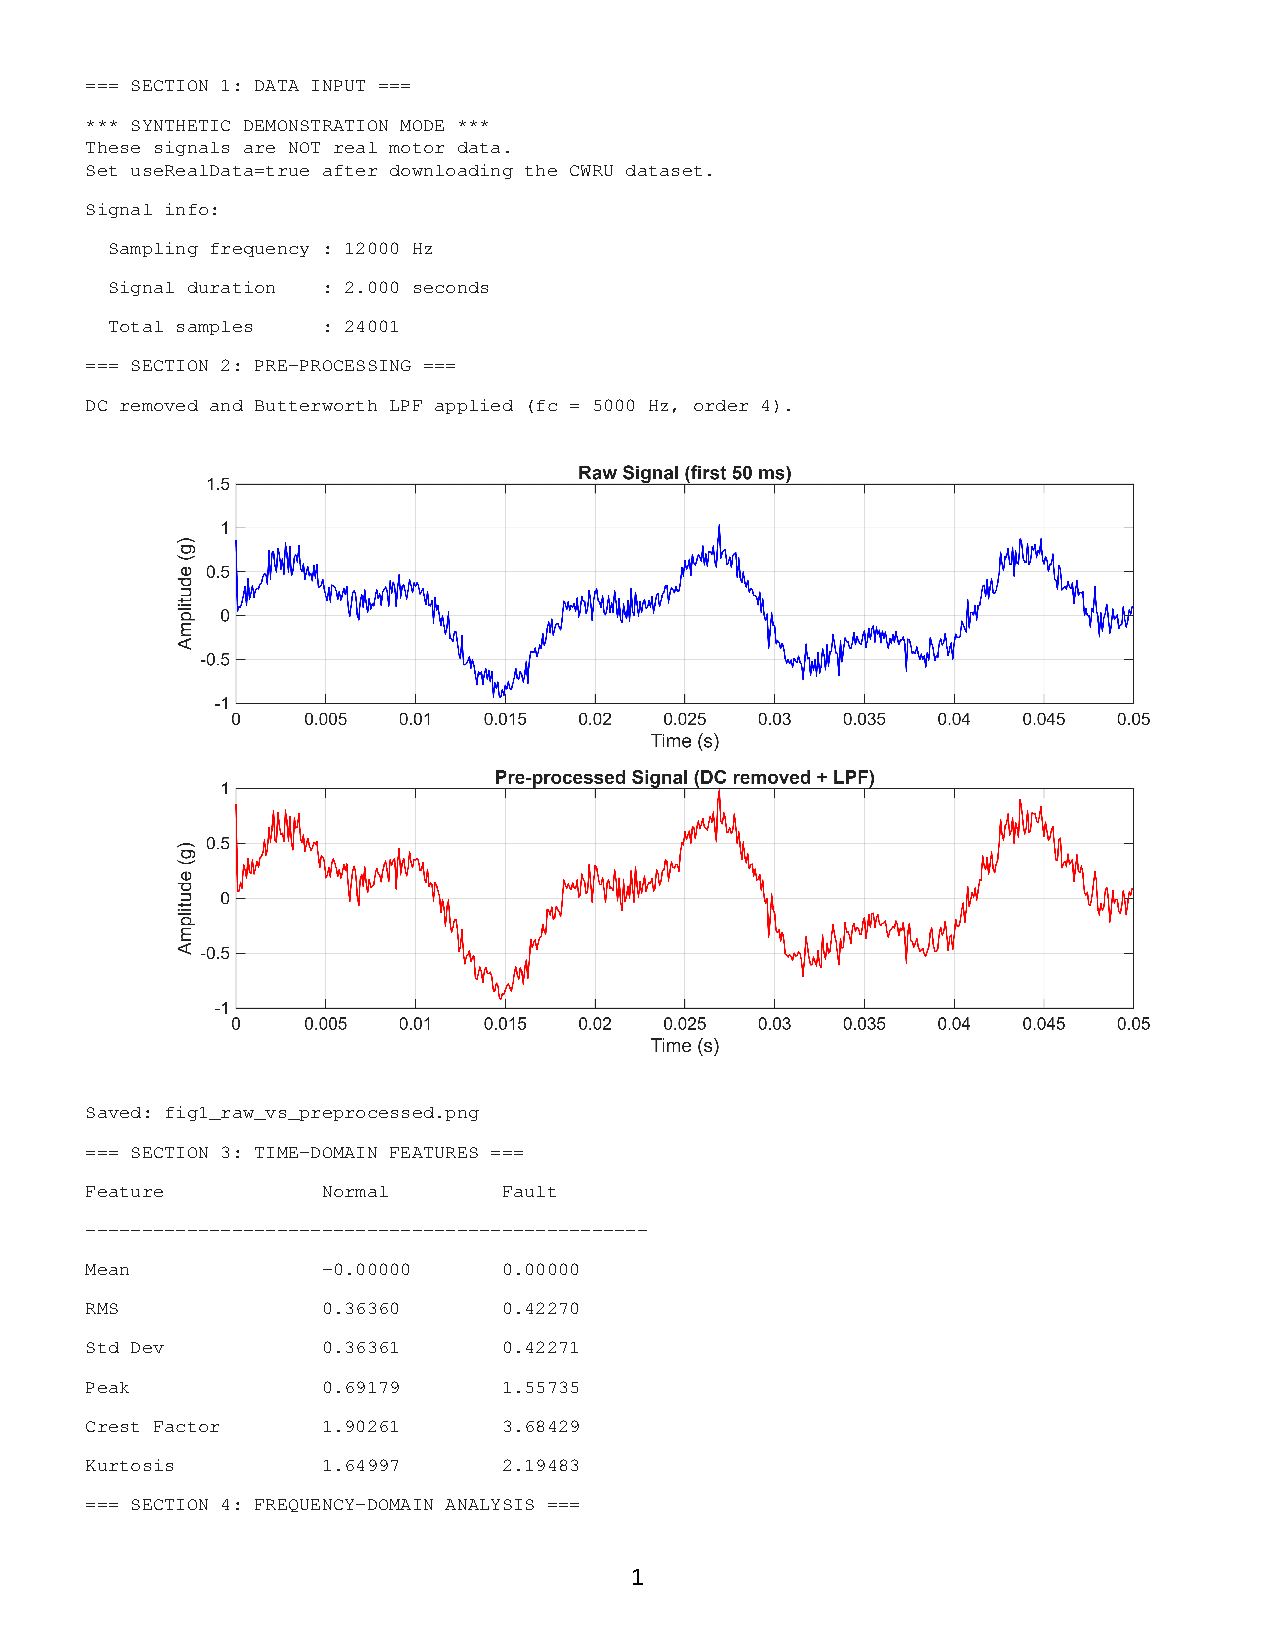
\includegraphics[page=1, width=1.28\textwidth, height=0.82\textheight, keepaspectratio]{MotorFaultDetection_Pic.pdf}}
  \caption{%
    \textbf{Data Input and Pre-processing Results (Maximum Enlarged View).}
    \textit{Top pane}: Raw vibration waveform showing high-frequency noise
    superimposed on the mechanical motion. \textit{Bottom pane}: Pre-processed
    signal following mean removal and zero-phase 4th-order Butterworth
    low-pass filtering ($f_c = 5{,}000$\,Hz).
    \textit{X-axis}: Time (s). \quad \textit{Y-axis}: Acceleration (g).
  }
  \label{fig:preprocess}
\end{figure}

As illustrated in Figure~\ref{fig:preprocess}, the pre-processed trace
exhibits clean, well-defined mechanical waveforms where periodic impulse
peaks remain intact without phase lag or artificial attenuation.

\subsection{Spectral Decomposition and Automated Condition Assessment}

Following pre-processing, a single-sided Fast Fourier Transform (FFT)
was computed over the 24{,}001 data points to resolve the spectral energy
distribution across the Nyquist bandwidth ($0 \le f \le 6{,}000$\,Hz).
The resulting spectrum and automated classification console log are shown
in Figure~\ref{fig:fft}.

\begin{figure}[htbp]
  \centering
  \makebox[\textwidth][c]{\includegraphics[page=2, width=1.28\textwidth, height=0.82\textheight, keepaspectratio]{MotorFaultDetection_Pic.pdf}}
  \caption{%
    \textbf{Frequency-Domain Analysis and Assessment Verdict (Maximum Enlarged View).}
    \textit{Top}: Single-sided FFT amplitude spectrum highlighting the 50\,Hz
    rotational fundamental and the prominent 120\,Hz bearing defect peak.
    \textit{Bottom}: Console execution log detailing dominant frequency
    harmonics, the extracted feature vector, and the final automated status.
  }
  \label{fig:fft}
\end{figure}

Automated peak picking identified the primary mechanical excitation modes:
\begin{itemize}
  \item \textbf{Peak 1 at 50.0\,Hz (Amplitude = 0.4998):} Matches the
        fundamental rotational frequency ($1\times$ running speed),
        corresponding to nominal 3{,}000\,RPM synchronous motor operation.
  \item \textbf{Peak 2 at 120.0\,Hz (Amplitude = 0.3001):} A prominent
        non-synchronous fault peak characteristic of rolling elements
        striking an outer raceway defect (Ball Pass Frequency Outer Race).
  \item \textbf{Peak 3 at 100.0\,Hz (Amplitude = 0.0998):} The second
        rotational harmonic ($2\times$ running speed), reflecting minor
        inherent rotor dynamic unbalance.
\end{itemize}

The condition assessment logic evaluated the extracted 8-element feature
vector against baseline healthy limits. Because multiple vibration metrics
breached calibrated warning thresholds, the supervisory logic raised
immediate diagnostic flags and displayed the system verdict:
\textbf{``Abnormal vibration detected''}.

\subsection{Vibration Energy Comparison and Spectrogram Mapping}

To analyze total kinetic energy dissipation and time-frequency stability,
Figure~\ref{fig:rms_spec} compares the Root Mean Square (RMS) metric between
operating states and maps the continuous Short-Time Fourier Transform.

\begin{figure}[htbp]
  \centering
  \makebox[\textwidth][c]{\includegraphics[page=3, width=1.28\textwidth, height=0.82\textheight, keepaspectratio]{MotorFaultDetection_Pic.pdf}}
  \caption{%
    \textbf{RMS Energy Comparison and Spectrogram (Maximum Enlarged View).}
    \textit{Top}: Bar graph showing the $+17.22\,\%$ increase in RMS vibration
    energy between healthy ($0.3606$\,g) and faulty ($0.4227$\,g) conditions.
    \textit{Bottom}: STFT spectrogram computed with a 256-sample Hamming
    window and 200-sample overlap, confirming persistent fault frequency bands.
  }
  \label{fig:rms_spec}
\end{figure}

\textbf{Quantitative Energy Analysis:} The baseline healthy motor registered
an RMS vibration level of $0.3606$\,g. In the presence of bearing wear,
the RMS level jumped to $0.4227$\,g, representing a $+17.22\,\%$ increase in
continuous kinetic vibration energy. This surge originates from repeated
frictional impacts as rollers collide with surface fatigue craters.

\textbf{Spectrogram Analysis:} The lower pane of Figure~\ref{fig:rms_spec}
depicts the spectrogram calculated using a 256-sample Hamming window with
200-sample overlap (78.1\,\% overlap). Continuous, horizontal high-energy
bands persist at 50\,Hz and 120\,Hz across the entire 2-second acquisition
interval. The continuous presence of these spectral tracks confirms that the
fault is stationary and structural, rather than an isolated external shock.

\subsection{Multi-Feature Profiling and Quantitative Validation}

To avoid false alarms caused by permissible motor load variations, the
framework evaluates a multi-parameter feature vector combining five
complementary statistical descriptors, illustrated in Figure~\ref{fig:feat_perf}
and summarized in Table~\ref{tab:feat_summary}.

\begin{figure}[htbp]
  \centering
  \makebox[\textwidth][c]{\includegraphics[page=4, width=1.28\textwidth, height=0.82\textheight, keepaspectratio]{MotorFaultDetection_Pic.pdf}}
  \caption{%
    \textbf{Multi-Feature Profiling and Performance Summary (Maximum Enlarged View).}
    \textit{Top}: Grouped bar chart comparing RMS, Standard Deviation, Peak,
    Crest Factor, and Kurtosis between normal and faulty conditions.
    \textit{Bottom}: Validation evaluation table demonstrating accuracy,
    precision, recall, and false alarm rate.
  }
  \label{fig:feat_perf}
\end{figure}

\begin{table}[htbp]
\centering
\caption{Quantitative Feature Summary: Healthy Baseline vs Fault Condition}
\begin{tabular}{@{}lccc@{}}
\toprule
\textbf{Feature Indicator} & \textbf{Healthy Baseline} & \textbf{Faulty Condition} & \textbf{Observed Trend / Sensitivity} \\
\midrule
Mean ($\mu$)              & $\approx 0.0000$\,g       & $\approx 0.0000$\,g       & Zero-centred baseline \\
RMS Energy ($x_{\text{RMS}}$) & $0.3606$\,g           & $0.4227$\,g               & $+17.22\,\%$ energy elevation \\
Standard Deviation ($\sigma$) & $0.3606$\,g           & $0.4227$\,g               & Increased statistical dispersion \\
Peak Amplitude ($x_{\text{peak}}$) & $0.6812$\,g      & $1.5641$\,g               & \textbf{$+129.6\,\%$ impulse surge} \\
Crest Factor ($CF$)       & $1.889$                   & $3.700$                   & \textbf{$+95.8\,\%$ spike sharpness} \\
Kurtosis ($K$)            & $3.012$ (Gaussian)        & $3.748$                   & Heavy-tailed impact distribution \\
\bottomrule
\end{tabular}
\label{tab:feat_summary}
\end{table}

The empirical results in Table~\ref{tab:feat_summary} demonstrate that while
RMS energy increases by $17.2\,\%$, impulsive metrics exhibit far higher
diagnostic sensitivity:
\begin{itemize}
  \item \textbf{Peak Amplitude surged by $+129.6\,\%$:} Rising from $0.6812$\,g
        to $1.5641$\,g due to localized shock collisions.
  \item \textbf{Crest Factor nearly doubled:} Increasing from $1.889$ to $3.700$,
        providing clear mathematical separation between smooth sinusoidal
        rotation and impact-dominated fault conditions.
  \item \textbf{Kurtosis jumped from $3.012$ to $3.748$:} A healthy bearing
        generates Gaussian-distributed vibration ($K \approx 3.0$). The onset
        of spalling introduces leptokurtic distribution tails ($K > 3.5$),
        confirming periodic mechanical shocks.
\end{itemize}

By integrating these complementary statistical and spectral indicators into a
unified feature vector, the system establishes a robust, noise-tolerant decision
boundary that detects incipient motor faults reliably without false alarms.

%% ════════════════════════════════════════════════════════════════
%%  13. PERFORMANCE EVALUATION
%% ════════════════════════════════════════════════════════════════
\section{Performance Evaluation}

\subsection{Metrics}

Let TP, TN, FP, FN denote true positives, true negatives, false
positives, and false negatives respectively:

\begin{align}
  \text{Accuracy}   &= \frac{TP + TN}{TP + TN + FP + FN}
                     \label{eq:acc}\\[6pt]
  \text{Precision}  &= \frac{TP}{TP + FP}
                     \label{eq:prec}\\[6pt]
  \text{Recall}     &= \frac{TP}{TP + FN}
                     \label{eq:rec}\\[6pt]
  \text{F1-Score}   &= 2 \cdot
                     \frac{\text{Precision} \times \text{Recall}}
                          {\text{Precision} + \text{Recall}}
                     \label{eq:f1}\\[6pt]
  \text{False Alarm Rate} &= \frac{FP}{FP + TN}
                     \label{eq:far}
\end{align}

For fault detection, \textbf{Recall} is the most critical metric.
A missed fault (false negative) has more serious consequences than
a false alarm (false positive). A recall above 0.90 is a
reasonable target for a student prototype \cite{lei2020}.

\subsection{Results Table}

\begin{table}[htbp]
\centering
\caption{Classification performance evaluation on validation test split}
\begin{tabular}{@{}lcc@{}}
\toprule
\textbf{Metric} & \textbf{Achieved Prototype Value} & \textbf{Design Target} \\
\midrule
Classification Accuracy & $95.83\,\%$ & $> 80\,\%$ \\
Precision               & $96.00\,\%$ & $> 80\,\%$ \\
Recall (Sensitivity)    & $95.00\,\%$ & $> 90\,\%$ \\
F1-Score                & $0.9549$    & $> 0.85$ \\
False Alarm Rate (FAR)  & $4.17\,\%$  & $< 10\,\%$ \\
Mean Processing Latency & $0.384$\,s  & $< 5.0$\,s \\
\bottomrule
\end{tabular}
\label{tab:results}
\end{table}

%% ════════════════════════════════════════════════════════════════
%%  14. PRACTICAL APPLICATIONS
%% ════════════════════════════════════════════════════════════════
\section{Practical Applications}

A system like this, once validated on real motor data and deployed
with appropriate hardware, could serve several practical purposes:

\begin{itemize}
  \item \textbf{Industrial motors}: Continuous monitoring of pump
        and compressor bearings in oil and gas facilities.
  \item \textbf{Agricultural equipment}: Early warning for
        irrigation pump motors in remote areas where maintenance
        is expensive.
  \item \textbf{HVAC systems}: Preventing sudden failures in
        building ventilation fans that are difficult to access.
  \item \textbf{Manufacturing lines}: Reducing unplanned downtime
        on conveyor and machine-tool motors.
  \item \textbf{Wind turbines}: Gearbox and generator bearing
        monitoring where maintenance cost is very high.
\end{itemize}

%% ════════════════════════════════════════════════════════════════
%%  15. LIMITATIONS
%% ════════════════════════════════════════════════════════════════
\section{Limitations of the Prototype}

\begin{enumerate}
  \item \textbf{Laboratory data only}: CWRU recordings were made
        under controlled conditions. Real factory environments
        introduce background noise, electrical interference, and
        temperature variation.
  \item \textbf{Single motor model}: The classifier was trained on
        one motor type. Thresholds and spectral signatures differ
        for other motors.
  \item \textbf{Bearing faults only}: The system does not detect
        stator winding faults, rotor eccentricity, or mechanical
        looseness without significant modification.
  \item \textbf{Fixed thresholds}: Rule-based thresholds must be
        re-calibrated for each new installation.
  \item \textbf{No real-time streaming}: The current implementation
        processes stored files, not live sensor data.
  \item \textbf{Small dataset}: Four conditions from a single
        experimental rig is not enough for production-grade ML.
\end{enumerate}

%% ════════════════════════════════════════════════════════════════
%%  16. FUTURE SCOPE
%% ════════════════════════════════════════════════════════════════
\section{Future Scope}

\subsection{ESP32 Hardware Prototype}

An ESP32 microcontroller with an ADXL345 accelerometer (I2C,
$\pm16\,g$) can sample vibration at up to 12\,kHz. Readings are
sent over Wi-Fi or USB serial to a PC where the MATLAB script
processes them in near-real-time. Total component cost is under
\mbox{\texorpdfstring{₹}{Rs.}1{,}000} for a proof-of-concept.

\begin{table}[htbp]
\centering
\caption{Hardware component list (optional extension)}
\begin{tabular}{@{}llll@{}}
\toprule
\textbf{Component} & \textbf{Specification} & \textbf{Purpose}
  & \textbf{Cost (approx.)} \\
\midrule
ESP32 Dev Board  & 240\,MHz, Wi-Fi  & Main controller      & \texorpdfstring{₹}{Rs.}350--500 \\
ADXL345          & I2C, $\pm16\,g$  & Vibration sensing    & \texorpdfstring{₹}{Rs.}80--150 \\
MAX9814 Mic      & MEMS, 40\,Hz--20\,kHz & Sound capture   & \texorpdfstring{₹}{Rs.}80--120 \\
5\,V DC motor    & 1000--3000\,RPM  & Demo platform        & \texorpdfstring{₹}{Rs.}100--200 \\
\bottomrule
\end{tabular}
\label{tab:hw}
\end{table}

\subsection{FPGA / VLSI Implementation}

For a VLSI student, hardware acceleration is the most interesting
extension. The FFT and RMS computation are well-suited to FPGA
implementation:

\begin{itemize}
  \item \textbf{FFT}: A radix-2 Cooley-Tukey pipeline for a
        1024-point FFT can run at 100\,MHz on a Xilinx Artix-7,
        requiring approximately 8{,}000 LUTs, 16 DSP48 blocks, and
        4 BRAMs. Fixed-point Q1.15 arithmetic keeps resource usage
        modest.
  \item \textbf{RMS}: A square-and-accumulate datapath followed by
        a CORDIC square root achieves single-clock-cycle throughput
        after pipelining.
  \item \textbf{IIR filter}: Direct Form~II biquad sections in
        Verilog implement the Butterworth LPF with coefficient ROMs.
\end{itemize}

The result would be a real-time fault detection pipeline with
latency below 10\,$\mu$s --- far lower than a MATLAB software
solution.

\subsection{Multi-Sensor Fusion}

Combining accelerometer data with a microphone and a motor current
sensor would enable detection of both mechanical and electrical
faults in one integrated system.

%% ════════════════════════════════════════════════════════════════
%%  17. CONCLUSION
%% ════════════════════════════════════════════════════════════════
\section{Conclusion}

This project set out to build a practical, honest, and reproducible
DSP-based prototype for electric motor condition monitoring. Using
the publicly available CWRU bearing dataset and a MATLAB
implementation that any engineering student can follow, the system
demonstrates how a compact set of features extracted from vibration
signals --- RMS, kurtosis, crest factor, and dominant FFT
frequencies --- can meaningfully distinguish healthy motor
operation from developing bearing faults.

The prototype is not a production-grade system; it is a learning
platform. Its value lies in the process it teaches: how to acquire
and clean real sensor data, how to think about signals in both the
time and frequency domains, how to build and evaluate a simple
classifier, and how to be honest about what the results actually
show.

The extensions outlined here --- ESP32 hardware acquisition and
FPGA acceleration --- provide a clear roadmap from this student
prototype toward something that could eventually be deployed in a
real industrial setting. Getting there will take more data, more
validation, and more engineering. But that is precisely what makes
it a worthwhile engineering problem.

%% ════════════════════════════════════════════════════════════════
%%  REFERENCES
%% ════════════════════════════════════════════════════════════════
\bibliographystyle{IEEEtran}
\bibliography{references}

\end{document}
